% !TeX program = pdflatex
%=======================================================================
%  Informe generado por tools/md2report.py
%  Compilar:  pdflatex informe.tex  (tres veces, por el indice)
%=======================================================================
\documentclass[11pt,a4paper]{article}

\usepackage[T1]{fontenc}
\usepackage[utf8]{inputenc}
\usepackage[spanish,es-noshorthands,es-tabla]{babel}
\usepackage{lmodern}
\usepackage[a4paper,top=2.5cm,bottom=2.4cm,left=2.8cm,right=2.5cm]{geometry}

\usepackage{xcolor}
\usepackage{graphicx}
\usepackage{booktabs}
\usepackage{longtable}
\usepackage{pdflscape}
\usepackage{array}
\usepackage{ragged2e}
\usepackage{enumitem}
\usepackage{amssymb}
\usepackage{titlesec}
\usepackage{fancyhdr}
\usepackage{parskip}
\usepackage{microtype}
\usepackage{caption}
\usepackage{etoolbox}
\usepackage[most]{tcolorbox}
\usepackage[hidelinks,breaklinks=true]{hyperref}
\usepackage{url}

\definecolor{navy}{HTML}{14496B}
\definecolor{sblue}{HTML}{2A78D6}
\definecolor{lblue}{HTML}{DCE8F4}
\definecolor{lgray}{HTML}{E6E8EA}
\definecolor{lamber}{HTML}{FBF1DE}
\definecolor{amber}{HTML}{A6690C}
\definecolor{red}{HTML}{B23B32}
\definecolor{green}{HTML}{2C6A49}
\definecolor{ink}{HTML}{18222E}
\definecolor{gray2}{HTML}{6D7885}
\definecolor{rule2}{HTML}{CFD5DC}
\definecolor{navybg}{HTML}{EFF4F9}
\definecolor{amberbg}{HTML}{FDF7EC}
\definecolor{redbg}{HTML}{FDF4F3}
\definecolor{greenbg}{HTML}{F1F7F3}

\hypersetup{colorlinks=true, linkcolor=navy, urlcolor=navy,
            citecolor=navy, pdftitle={Selección del LED para el módulo de iluminación compacto}}
\renewcommand{\UrlFont}{\small\ttfamily}
\Urlmuskip=0mu plus 1mu
\def\UrlBreaks{\do\/\do\-\do\_\do\.\do\=\do\&\do\?\do\#\do\:\do\0\do\1\do\2\do\3\do\4\do\5\do\6\do\7\do\8\do\9}
\sloppy

\newlength{\colw}
\newcolumntype{L}{>{\RaggedRight\arraybackslash}p{\colw}}
\renewcommand{\arraystretch}{1.3}
\setlist{topsep=3pt, itemsep=1.5pt, parsep=0pt, leftmargin=1.4em}
\captionsetup{skip=4pt}

% --- titulos ----------------------------------------------------------
\titleformat{\section}
  {\sffamily\LARGE\bfseries\color{navy}}{}{0pt}{}
  [\vspace{2pt}{\color{navy}\titlerule[1.4pt]}]
\titleformat{\subsection}{\sffamily\large\bfseries}{}{0pt}{}
  [\vspace{1pt}{\color{rule2}\titlerule[0.5pt]}]
\titleformat{\subsubsection}{\sffamily\normalsize\bfseries\color{navy}}{}{0pt}{}
\titleformat{\paragraph}[runin]{\sffamily\small\bfseries\color{gray2}}{}{0pt}{}[\quad]
\titlespacing*{\section}{0pt}{0pt}{14pt}
\titlespacing*{\subsection}{0pt}{18pt}{7pt}
\titlespacing*{\subsubsection}{0pt}{13pt}{4pt}

\pagestyle{fancy}
\fancyhf{}
\renewcommand{\headrulewidth}{0.4pt}
\fancyhead[L]{\sffamily\footnotesize\color{gray2}Memoria técnica — Selección del LED OSLON SSL 80 (GW CS8PM1.PM)}
\fancyfoot[C]{\sffamily\footnotesize\thepage}

% --- distintivos ------------------------------------------------------
\newcommand{\badge}[3]{%
  \tcbox[on line, boxsep=1pt, left=2pt, right=2pt, top=0.5pt, bottom=0.5pt,
         colback=#1, colframe=#1, arc=1pt, boxrule=0pt]%
    {\color{#2}\sffamily\scriptsize\bfseries #3}}

% --- llamados ---------------------------------------------------------
\newtcolorbox{notaclavebase}{enhanced, breakable, sharp corners, boxrule=0pt,
  leftrule=2.5pt, colframe=amber, colback=amberbg,
  left=8pt, right=8pt, top=7pt, bottom=7pt, before skip=10pt, after skip=10pt}
\newenvironment{notaclave}[1]
  {\begin{notaclavebase}{\sffamily\scriptsize\bfseries\color{amber}#1}\par\vspace{2pt}}
  {\end{notaclavebase}}
\newtcolorbox{notadatobase}{enhanced, breakable, sharp corners, boxrule=0pt,
  leftrule=2.5pt, colframe=navy, colback=navybg,
  left=8pt, right=8pt, top=7pt, bottom=7pt, before skip=10pt, after skip=10pt}
\newenvironment{notadato}[1]
  {\begin{notadatobase}{\sffamily\scriptsize\bfseries\color{navy}#1}\par\vspace{2pt}}
  {\end{notadatobase}}
\newtcolorbox{notariesgobase}{enhanced, breakable, sharp corners, boxrule=0pt,
  leftrule=2.5pt, colframe=red, colback=redbg,
  left=8pt, right=8pt, top=7pt, bottom=7pt, before skip=10pt, after skip=10pt}
\newenvironment{notariesgo}[1]
  {\begin{notariesgobase}{\sffamily\scriptsize\bfseries\color{red}#1}\par\vspace{2pt}}
  {\end{notariesgobase}}
\newtcolorbox{notainferenciabase}{enhanced, breakable, sharp corners, boxrule=0pt,
  leftrule=2.5pt, colframe=green, colback=greenbg,
  left=8pt, right=8pt, top=7pt, bottom=7pt, before skip=10pt, after skip=10pt}
\newenvironment{notainferencia}[1]
  {\begin{notainferenciabase}{\sffamily\scriptsize\bfseries\color{green}#1}\par\vspace{2pt}}
  {\end{notainferenciabase}}

% --- tarjetas ---------------------------------------------------------
\newtcolorbox{tarjetabase}{enhanced, breakable, colframe=rule2, colback=white,
  boxrule=0.6pt, arc=2pt, left=8pt, right=8pt, top=6pt, bottom=6pt,
  before skip=8pt, after skip=8pt}
\newenvironment{tarjeta}[2]
  {\begin{tarjetabase}%
   {\sffamily\bfseries\color{navy}#1}%
   \ifstrempty{#2}{}{\\[1pt]{\sffamily\scriptsize\color{gray2}#2}}%
   \par\vspace{3pt}}
  {\end{tarjetabase}}

% --- desplegables (siempre visibles en papel) -------------------------
\newtcolorbox{detallebase}[1]{enhanced, breakable, colframe=rule2,
  colback=white, boxrule=0.6pt, arc=2pt, left=8pt, right=8pt, top=6pt,
  bottom=6pt, before skip=10pt, after skip=10pt,
  title={\sffamily\small\bfseries #1}, colbacktitle=navybg, coltitle=navy,
  titlerule=0pt}
\newenvironment{detalle}[1]{\begin{detallebase}{#1}}{\end{detallebase}}

\begin{document}
\pagenumbering{roman}

\begin{titlepage}
\thispagestyle{empty}
\setlength{\parindent}{0pt}\raggedright
\vspace*{3cm}
{\sffamily\footnotesize\bfseries\color{navy}\MakeUppercase{Memoria técnica \textperiodcentered{} Selección de componente}\par}
\vspace{8pt}
{\color{navy}\rule{\linewidth}{2.5pt}}
\vspace{22pt}

{\sffamily\huge\bfseries Selección del LED para el módulo de iluminación compacto\par}
\vspace{14pt}
{\sffamily\large\color{gray2} OSRAM OSLON SSL 80 \textperiodcentered{} GW CS8PM1.PM, 5000 K, bin LUMQ — robot de almacenamiento de medicamentos para farmacia\par}
\vspace{30pt}
{\color{rule2}\rule{0.35\linewidth}{0.6pt}\par}
\vspace{12pt}
{\normalsize Datos técnicos y de distribuidores verificados el 27 de septiembre de 2026\par}
\vfill
{\sffamily\footnotesize\color{gray2}Memoria de selección de componente. Los valores de flujo de salida son estimaciones de cálculo con supuestos declarados; deben confirmarse con medición sobre prototipo antes de congelar el diseño. Precios y stock se verificaron el 27-09-2026 y deben revisarse antes de cada compra.\par}
\end{titlepage}
\setcounter{page}{2}

\tableofcontents
\clearpage
\pagenumbering{arabic}

\clearpage

\section*{Resumen ejecutivo}
\addcontentsline{toc}{section}{Resumen ejecutivo}

Para el módulo de iluminación compacto del robot de almacenamiento de medicamentos se selecciona el LED \textbf{ams OSRAM OSLON SSL 80, tipo GW CS8PM1.PM, variante 5000 K bin LUMQ} (códigos GW CS8PM1.PM-LUMQ-XX53-1 o -A333-1), que entrega \textbf{164 a 210 lm a 350 mA} con un consumo cercano a \textbf{1 W}.

La elección responde a la geometría: el LED queda al fondo de un conducto de aluminio fresado, a \textbf{7 mm} de una ventana de \textbf{Ø 5 mm}. En ese espacio, un encapsulado de 3,0 $\times$ 3,0 mm con cono preenfocado de \textbf{80\textdegree{}} entrega a la ventana casi el doble de luz directa que un LED típico de 120\textdegree{} (19,4 \% contra 11,3 \% del flujo total), con paquete cerámico, resistencia térmica de 3,7 K/W y rango industrial de $-$40 a +125 \textdegree{}C.

El objetivo de \textbf{100 lm útiles a la salida es alcanzable pero no está garantizado}. Solo con luz directa llegan a la ventana 32–41 lm. El resultado final depende sobre todo de cómo refleja la pared interna: con aluminio que conserve componente especular y un difusor de alta transmisión se obtienen \textbf{95–140 lm}; con una pared mate y difusa el rango cae a \textbf{40–80 lm}. La recomendación es prototipar y medir, y dejar previsto un tratamiento de la pared (pulido, inserto o recubrimiento reflectivo) como medida de recuperación.

\begin{center}\setlength{\tabcolsep}{4pt}
\begin{tabular}{>{\raggedright\arraybackslash}p{0.230\linewidth}>{\raggedright\arraybackslash}p{0.230\linewidth}>{\raggedright\arraybackslash}p{0.230\linewidth}>{\raggedright\arraybackslash}p{0.230\linewidth}}
{\color{navy}\Large\bfseries 164–210 lm}\par\vspace{2pt}{\small flujo del bin LUMQ a 350 mA}\par\vspace{1pt}{\footnotesize\color{gray2} 5000 K, CRI $\geq$ 70} & {\color{navy}\Large\bfseries $\approx$ 1,0 W}\par\vspace{2pt}{\small potencia eléctrica típica}\par\vspace{1pt}{\footnotesize\color{gray2} 350 mA $\times$ 2,85 V} & {\color{navy}\Large\bfseries 19,4 \%}\par\vspace{2pt}{\small del flujo llega directo a la ventana}\par\vspace{1pt}{\footnotesize\color{gray2} geometría Ø 5 mm a 7 mm} & {\color{navy}\Large\bfseries 40–140 lm}\par\vspace{2pt}{\small rango estimado a la salida}\par\vspace{1pt}{\footnotesize\color{gray2} según pared y difusor} \\
\end{tabular}\end{center}
\begin{notaclave}{Decisión}
\textbf{Se recomienda el OSLON SSL 80 GW CS8PM1.PM-LUMQ-XX53-1 (5000 K), alimentado a 350 mA con fuente de corriente constante.} La decisión del componente es firme; lo que queda abierto es la \textbf{eficiencia del conducto}, que se resuelve con una medición sobre prototipo y no cambiando de LED.

\end{notaclave}

\subsection*{Requisitos del sistema frente al LED seleccionado}
\addcontentsline{toc}{subsection}{Requisitos del sistema frente al LED seleccionado}

\begingroup\footnotesize
\setlength{\tabcolsep}{4pt}
\setlength{\emergencystretch}{4em}
\hyphenpenalty=50 \exhyphenpenalty=50
\begin{longtable}{@{}>{\RaggedRight\arraybackslash}p{\dimexpr 0.3012\linewidth-2\tabcolsep\relax}>{\RaggedRight\arraybackslash}p{\dimexpr 0.2490\linewidth-2\tabcolsep\relax}>{\RaggedRight\arraybackslash}p{\dimexpr 0.2490\linewidth-2\tabcolsep\relax}>{\RaggedRight\arraybackslash}p{\dimexpr 0.1958\linewidth-2\tabcolsep\relax}@{}}
\toprule
\scriptsize\textbf{Requisito del sistema} & \scriptsize\textbf{Valor pedido} & \scriptsize\textbf{OSLON SSL 80, LUMQ 5000 K} & \scriptsize\textbf{Cumplimiento} \\
\midrule
\endfirsthead
\toprule
\scriptsize\textbf{Requisito del sistema} & \scriptsize\textbf{Valor pedido} & \scriptsize\textbf{OSLON SSL 80, LUMQ 5000 K} & \scriptsize\textbf{Cumplimiento} \\
\midrule
\endhead
\bottomrule
\endfoot
Encapsulado compatible con alojamiento mecanizado & LED SMD compacto & 3,0 $\times$ 3,0 mm, altura 2,13–2,30 mm, cerámico & Cumple \\
Concentrar la luz hacia una ventana de Ø 5 mm a 7 mm & Cono estrecho & 2$\varphi$ = 80\textdegree{} a 50 \% de intensidad & Cumple \\
Flujo disponible en el LED & Muy superior a 100 lm, para cubrir pérdidas & 164–210 lm a 350 mA & Cumple \\
100 lm útiles a la salida & $\approx$ 100 lm & 40–140 lm según pared y difusor & \textbf{A verificar} \\
Operación continua 24/7 & Robustez térmica & RthJS 3,7 K/W; Top $-$40 a +125 \textdegree{}C & Cumple con diseño térmico \\
Alimentación simple y controlable & Driver estándar & Corriente constante 350 mA, Vf 2,70–3,20 V & Cumple \\
Observación, cámara, detección & Luz blanca estable & 5000 K, CRI 70 mín. & Cumple (no colorimetría) \\
Industrialización & Montaje automático & SMD en carrete de 600, MSL 2 & Cumple \\
Abastecimiento & Disponible en distribución & Stock en Mouser Europa (1.669 u.) & Cumple, con importación \\
\end{longtable}
\endgroup

\clearpage

\section*{Parte I — El componente}
\addcontentsline{toc}{section}{Parte I — El componente}


\subsection*{1. Contexto y restricciones del sistema}
\addcontentsline{toc}{subsection}{1. Contexto y restricciones del sistema}

El módulo ilumina el interior del robot para observación, cámara o detección. La mecánica impone condiciones que ordenan toda la selección:

\begin{itemize}
\item LED SMD de alta potencia dentro de un alojamiento mecanizado.
\item Distancia aproximada entre el LED y la ventana o difusor: \textbf{7 mm}.
\item Ventana circular de salida de \textbf{Ø 5 mm}, con difusor.
\item Conducto interno de \textbf{aluminio mecanizado o fresado}, con buena terminación pero \textbf{no pulido}.
\item Objetivo de salida: del orden de \textbf{100 lm útiles}.
\end{itemize}

\begin{figure}[htbp]\centering
\fbox{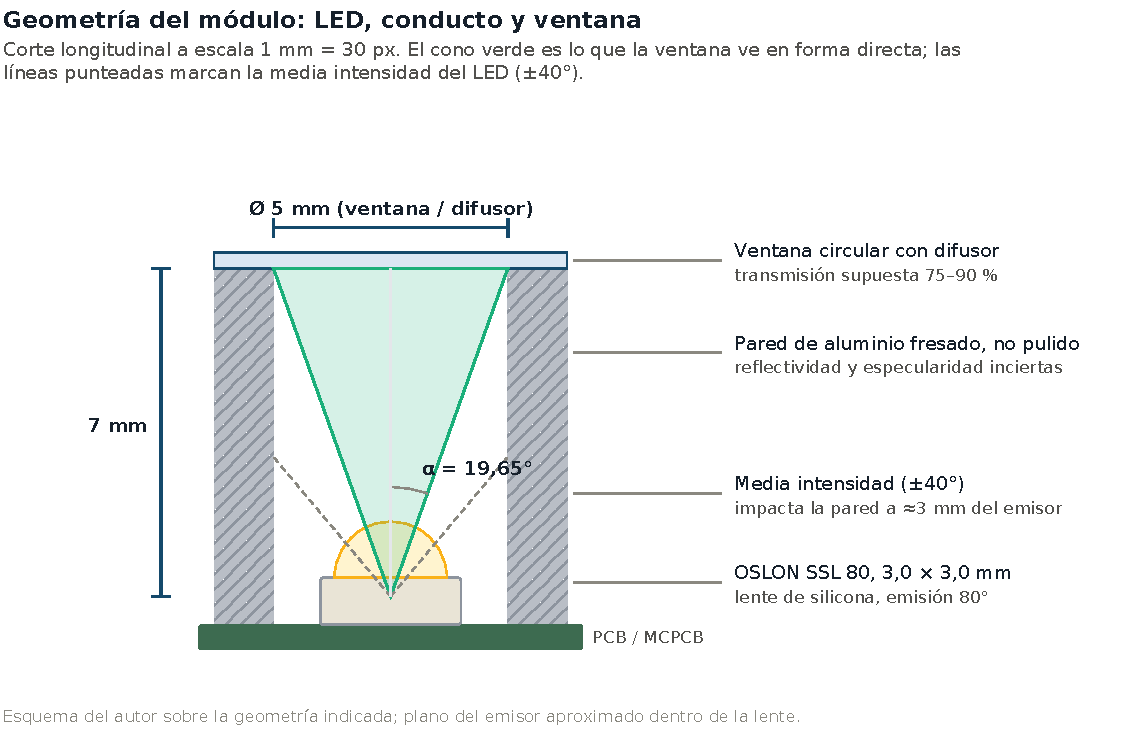
\includegraphics[width=0.88\linewidth]{assets/led-geometria.pdf}}
\caption*{\footnotesize\raggedright Figura 1 — Geometría del módulo. El cono verde es la luz que llega a la ventana sin tocar la pared; todo lo que sale fuera de él depende de la pared para llegar. {\color{gray2}Esquema del autor.}}
\end{figure}
\begin{notariesgo}{La pared del conducto es la variable crítica}
Un aluminio fresado sin pulir \textbf{no debe modelarse como espejo}. Puede conservar parte de la reflexión especular, pero la rugosidad, las marcas de fresa, la oxidación y la limpieza de la superficie pueden bajar mucho la eficiencia óptica. En este diseño, esa superficie pesa más en el resultado final que la elección entre bins del LED.

\end{notariesgo}

\subsection*{2. LED seleccionado}
\addcontentsline{toc}{subsection}{2. LED seleccionado}

\begingroup\footnotesize
\setlength{\tabcolsep}{4pt}
\setlength{\emergencystretch}{4em}
\hyphenpenalty=50 \exhyphenpenalty=50
\begin{longtable}{@{}>{\RaggedRight\arraybackslash}p{\dimexpr 0.3404\linewidth-2\tabcolsep\relax}>{\RaggedRight\arraybackslash}p{\dimexpr 0.6546\linewidth-2\tabcolsep\relax}@{}}
\toprule
\scriptsize\textbf{Campo} & \scriptsize\textbf{Valor} \\
\midrule
\endfirsthead
\toprule
\scriptsize\textbf{Campo} & \scriptsize\textbf{Valor} \\
\midrule
\endhead
\bottomrule
\endfoot
Fabricante & ams OSRAM \\
Familia & OSRAM OSLON SSL 80 \\
Tipo base & GW CS8PM1.PM \\
Variante preferida & \textbf{GW CS8PM1.PM-LUMQ-XX53-1} (Q65113A9964) o \textbf{GW CS8PM1.PM-LUMQ-A333-1} (Q65113A9963) \\
Temperatura de color & 5000 K \\
Flujo a 350 mA & 164 a 210 lm (grupos LU, MP y MQ) \\
Código en distribución & GW CS8PM1.PM-LUMQ-XX53-1-350-R18 (carrete de 600 unidades) \\
Estado & \emph{Full production} según la página oficial del producto \\
\end{longtable}
\endgroup

El bin \textbf{LUMQ} es el de mayor flujo listado para 5000 K en la versión vigente del datasheet (v1.10, 2026-03-05). Las dos variantes, XX53 y A333, comparten flujo y temperatura de color; solo difieren en la agrupación cromática del pedido, que el datasheet codifica en el sufijo.

\begin{figure}[htbp]\centering
\fbox{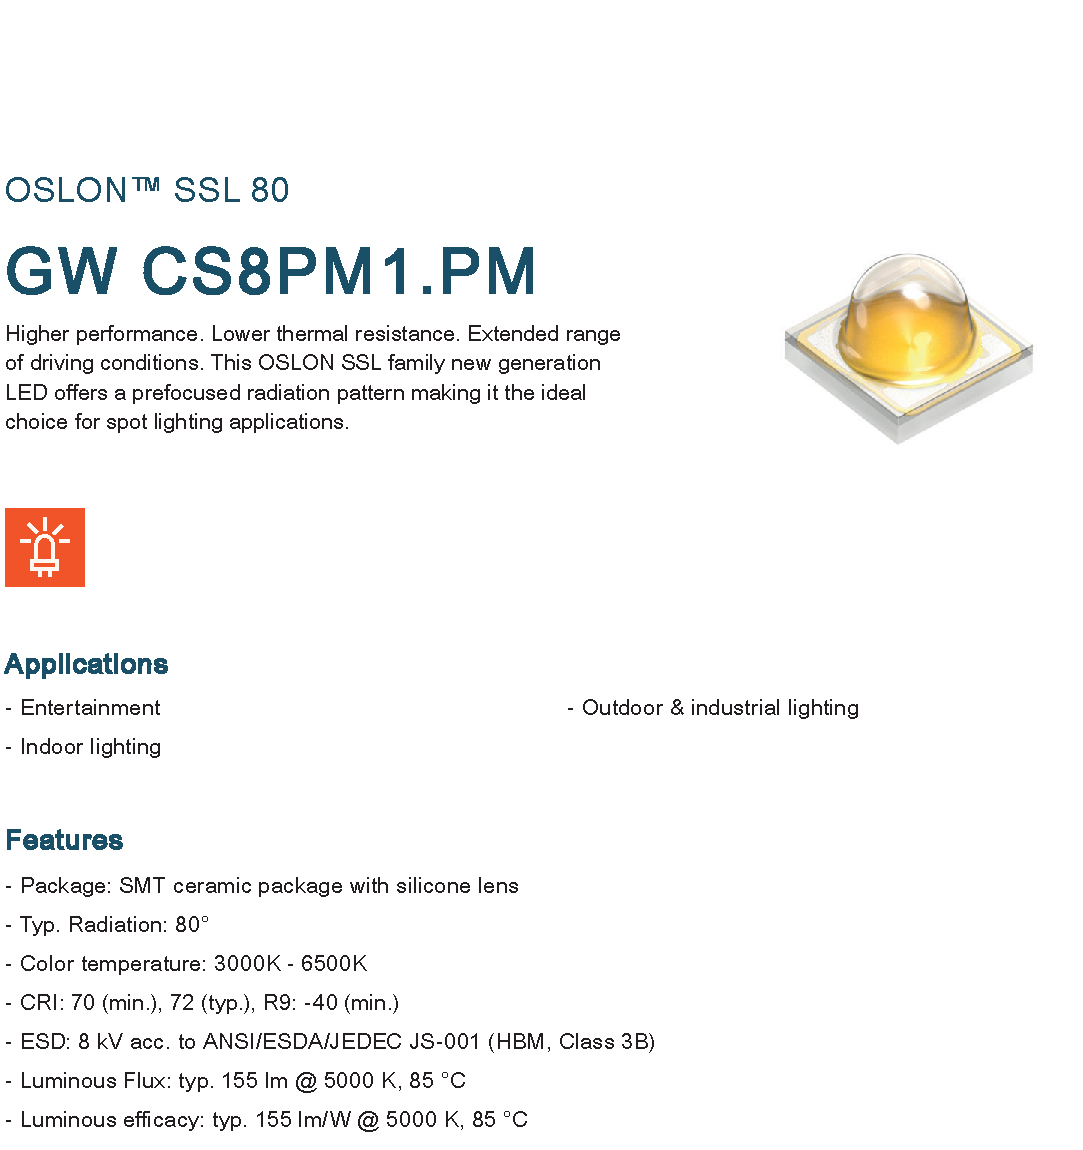
\includegraphics[width=0.71\linewidth]{assets/led-ds-portada.pdf}}
\caption*{\footnotesize\raggedright Figura 2 — Resumen del componente: encapsulado cerámico con lente de silicona, radiación típica de 80\textdegree{}, CRI 70 mín. y aplicaciones previstas. {\color{gray2}Fuente: ams OSRAM, datasheet GW CS8PM1.PM, versión 1.10, 2026-03-05, p. 2.}}
\end{figure}
\begin{figure}[htbp]\centering
\fbox{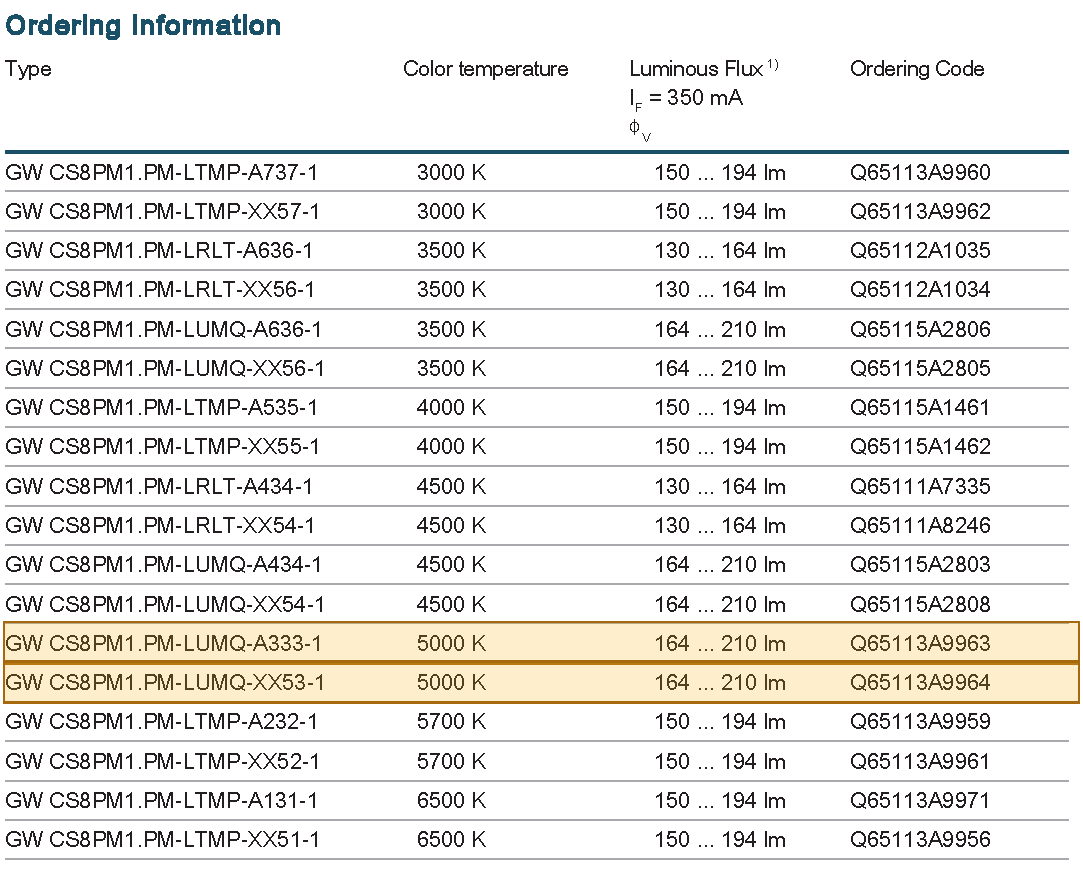
\includegraphics[width=0.88\linewidth]{assets/led-ds-pedido.pdf}}
\caption*{\footnotesize\raggedright Figura 3 — Tabla de pedido. Resaltadas, las dos variantes LUMQ de 5000 K con 164 a 210 lm a 350 mA. {\color{gray2}Fuente: ams OSRAM, datasheet GW CS8PM1.PM, versión 1.10, 2026-03-05, p. 3.}}
\end{figure}

\subsection*{3. Por qué este LED y no otro}
\addcontentsline{toc}{subsection}{3. Por qué este LED y no otro}

\begin{tarjeta}{LED de 120\textdegree{} a 150\textdegree{}}{Descartado}
Es lo más común en LEDs blancos de potencia. Con una ventana tan chica, \textbf{desperdicia más luz contra las paredes}: en $\alpha$ = 19,65\textdegree{} un LED lambertiano de 120\textdegree{} entrega directo el 11,3 \% de su flujo y uno de 150\textdegree{}, el 8,7 \%. Todo lo demás queda a merced del aluminio.

\end{tarjeta}
\begin{tarjeta}{LED o lente muy cerrados}{Descartado}
Un haz de 30\textdegree{} a 60\textdegree{} mete más luz directa, pero genera un \textbf{punto caliente más fuerte} sobre el difusor y vuelve el módulo \textbf{dependiente de la alineación} entre LED y conducto. Suma además una óptica secundaria que no entra en el alojamiento.

\end{tarjeta}
\begin{tarjeta}{OSLON SSL 80}{Seleccionado}
Es el \textbf{compromiso} entre tamaño, flujo, disponibilidad industrial y cono preenfocado: \textbf{19,4 \%} de captura directa, 164–210 lm en 3 $\times$ 3 mm, paquete cerámico y una familia en producción plena con distribución internacional.

\end{tarjeta}
\begin{figure}[htbp]\centering
\fbox{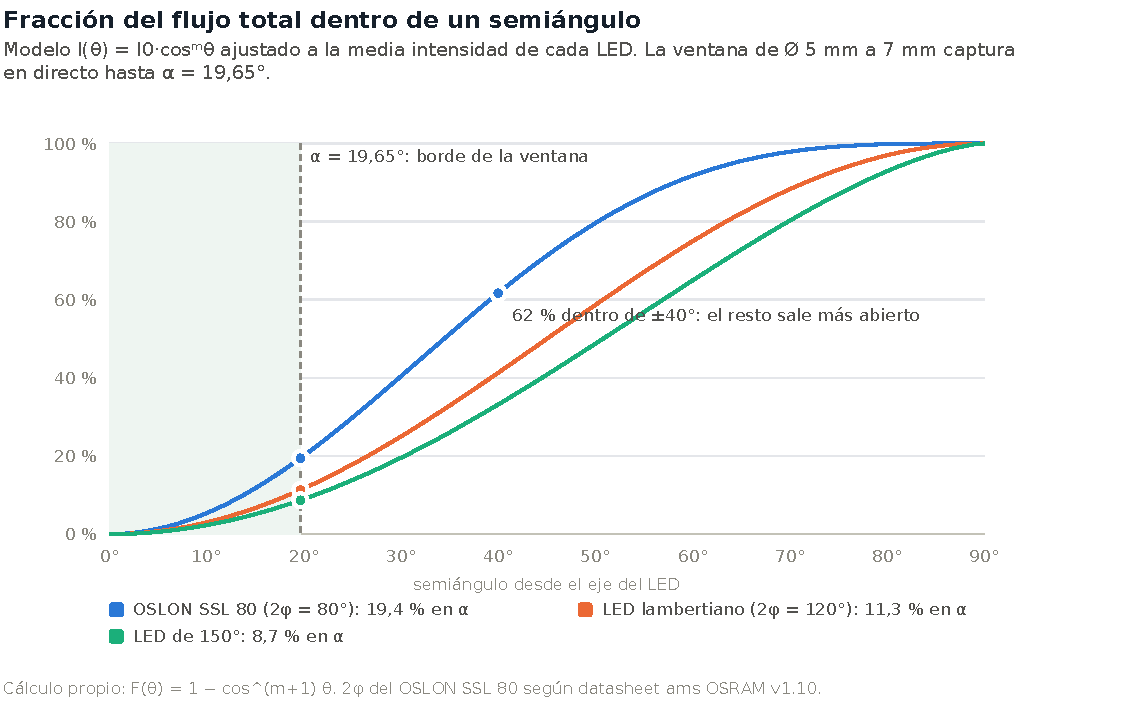
\includegraphics[width=0.88\linewidth]{assets/led-captura.pdf}}
\caption*{\footnotesize\raggedright Figura 4 — Fracción del flujo total que sale dentro de cada semiángulo. En el borde de la ventana (19,65\textdegree{}) el OSLON SSL 80 captura en directo 1,7 veces lo que un LED de 120\textdegree{} y 2,2 veces lo que uno de 150\textdegree{}. {\color{gray2}Cálculo propio con modelo cos\textsuperscript{m}$\theta$; 2$\varphi$ del OSLON SSL 80 según el datasheet ams OSRAM v1.10.}}
\end{figure}
Frente a \textbf{LEDs genéricos} de encapsulado plástico (PLCC, 2835, 5050), el OSLON SSL 80 aporta un paquete cerámico con resistencia térmica baja, ficha técnica completa con curvas de derating, agrupación por flujo, tensión y color, trazabilidad de lote y gestión de cambios de producto. Para un equipo 24/7 en un entorno regulado, esa documentación es parte del valor del componente.

\clearpage

\section*{Parte II — Características}
\addcontentsline{toc}{section}{Parte II — Características}


\subsection*{4. Características eléctricas, ópticas, térmicas y mecánicas}
\addcontentsline{toc}{subsection}{4. Características eléctricas, ópticas, térmicas y mecánicas}

Valores a IF = 350 mA y Tj = 85 \textdegree{}C, salvo indicación.

\begingroup\footnotesize
\setlength{\tabcolsep}{4pt}
\setlength{\emergencystretch}{4em}
\hyphenpenalty=50 \exhyphenpenalty=50
\begin{longtable}{@{}>{\RaggedRight\arraybackslash}p{\dimexpr 0.1783\linewidth-2\tabcolsep\relax}>{\RaggedRight\arraybackslash}p{\dimexpr 0.2377\linewidth-2\tabcolsep\relax}>{\RaggedRight\arraybackslash}p{\dimexpr 0.2819\linewidth-2\tabcolsep\relax}>{\RaggedRight\arraybackslash}p{\dimexpr 0.2971\linewidth-2\tabcolsep\relax}@{}}
\toprule
\scriptsize\textbf{Grupo} & \scriptsize\textbf{Parámetro} & \scriptsize\textbf{Valor} & \scriptsize\textbf{Nota} \\
\midrule
\endfirsthead
\toprule
\scriptsize\textbf{Grupo} & \scriptsize\textbf{Parámetro} & \scriptsize\textbf{Valor} & \scriptsize\textbf{Nota} \\
\midrule
\endhead
\bottomrule
\endfoot
Eléctrico & Tensión directa Vf & 2,70 mín. \textperiodcentered{} \textbf{2,85 típ.} \textperiodcentered{} 3,20 máx. V & Grupos K2 a M2, de 0,10 V \\
Eléctrico & Corriente directa & 100 mA mín. \textperiodcentered{} 1300 mA máx. & Punto de diseño: 350 mA \\
Eléctrico & Corriente de pico & 2000 mA & t $\leq$ 10 $\mu$s, D = 0,005 \\
Eléctrico & Potencia típica & $\approx$ 1,0 W & 0,35 A $\times$ 2,85 V \\
Eléctrico & Tensión inversa & 1,2 V máx. (IR = 20 mA) & No polarizar en inversa \\
Eléctrico & ESD & 8 kV HBM, clase 3B & Diodo de protección en paralelo al chip \\
Óptico & Ángulo de emisión 2$\varphi$ & 80\textdegree{} a 50 \% de intensidad & Semiángulo de 40\textdegree{} \\
Óptico & Flujo, bin LUMQ & 164–210 lm & Tolerancia de medición $\pm$7 \% \\
Óptico & Temperatura de color & 5000 K &  \\
Óptico & CRI / R9 & 70 mín., 72 típ. / $-$40 mín. &  \\
Térmico & RthJS eléctrica & 3,7 K/W típ. & Con eficiencia $\eta$e = 30 \% \\
Térmico & Temperatura de juntura & 135 \textdegree{}C máx. (160 \textdegree{}C absoluta) &  \\
Térmico & Temperatura de operación & $-$40 a +125 \textdegree{}C & Igual para almacenamiento \\
Mecánico & Cuerpo & 3,0 $\times$ 3,0 mm (2,9–3,1) &  \\
Mecánico & Altura total & 2,13–2,30 mm & Plano del datasheet, p. 16 \\
Mecánico & Peso & 22,3 mg &  \\
Proceso & Sensibilidad a la humedad & MSL 2 (JEDEC J-STD-020E) & Reflow sin plomo, pico 245–250 \textdegree{}C \\
Proceso & Embalaje & Cinta, carrete Ø 180 mm, 600 unidades &  \\
\end{longtable}
\endgroup

\begin{notadato}{Corrección sobre la altura del encapsulado}
El plano dimensional oficial acota la altura total entre \textbf{2,13 y 2,30 mm}. En la documentación de partida figuraba 2,21–2,30 mm; para el diseño mecánico del alojamiento debe usarse el rango completo del plano.

\end{notadato}
\begin{figure}[htbp]\centering
\fbox{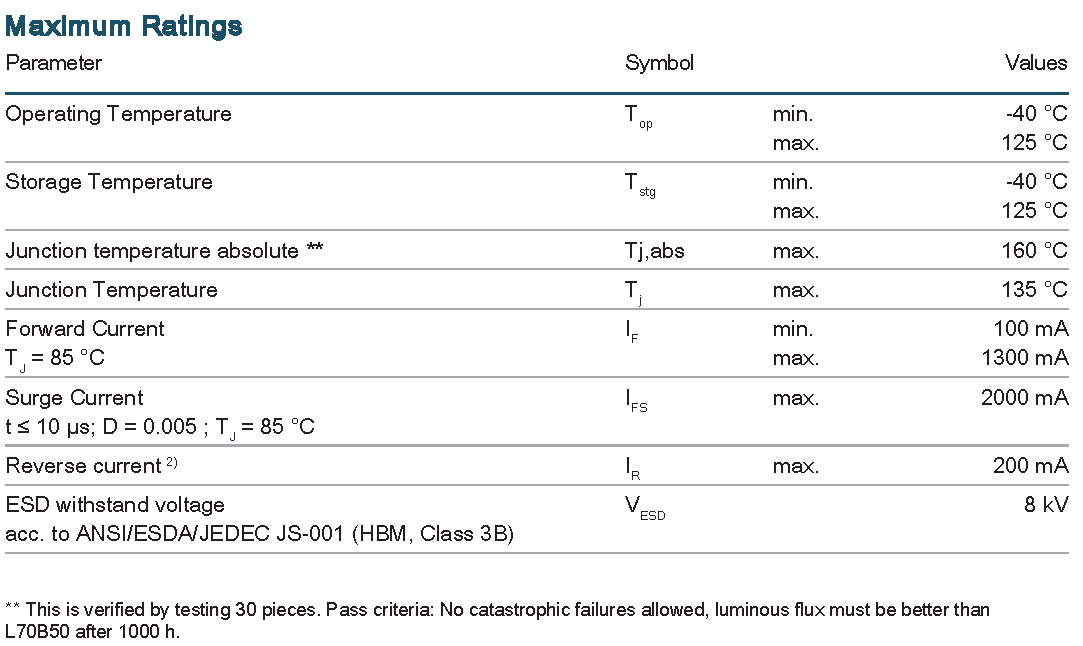
\includegraphics[width=0.88\linewidth]{assets/led-ds-maximos.pdf}}
\caption*{\footnotesize\raggedright Figura 5 — Valores máximos: corriente directa de 100 a 1300 mA, juntura de 135 \textdegree{}C, operación de $-$40 a +125 \textdegree{}C y ESD de 8 kV. {\color{gray2}Fuente: ams OSRAM, datasheet GW CS8PM1.PM, versión 1.10, 2026-03-05, p. 4.}}
\end{figure}
\begin{figure}[htbp]\centering
\fbox{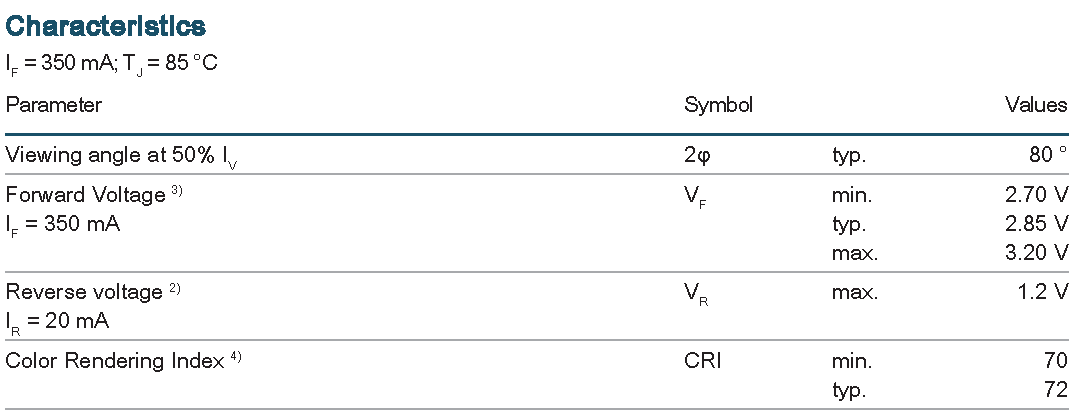
\includegraphics[width=0.88\linewidth]{assets/led-ds-caracteristicas.pdf}}
\caption*{\footnotesize\raggedright Figura 6 — Características a 350 mA y 85 \textdegree{}C: 80\textdegree{}, Vf 2,70/2,85/3,20 V, CRI 70/72 y RthJS 3,7 K/W. {\color{gray2}Fuente: ams OSRAM, datasheet GW CS8PM1.PM, versión 1.10, 2026-03-05, p. 5.}}
\end{figure}
\begin{figure}[htbp]\centering
\fbox{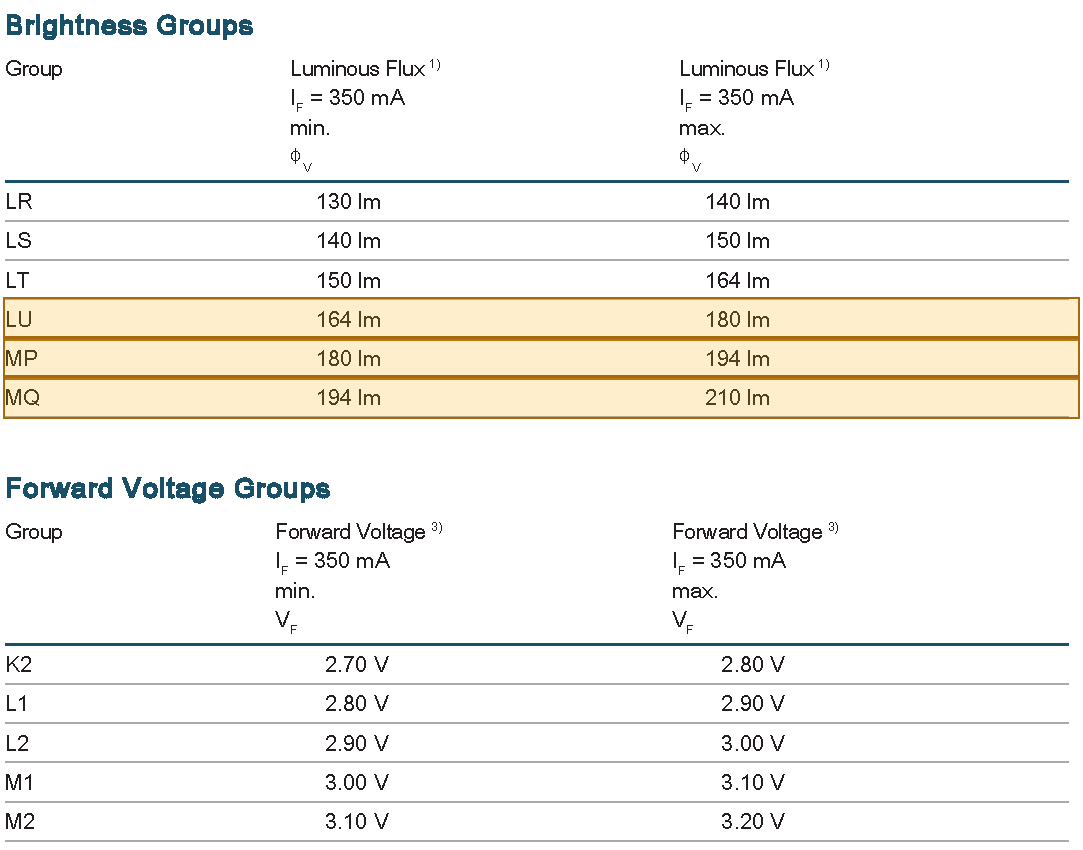
\includegraphics[width=0.83\linewidth]{assets/led-ds-grupos.pdf}}
\caption*{\footnotesize\raggedright Figura 7 — Grupos de flujo y de tensión directa. Resaltados, los grupos LU, MP y MQ que componen el bin LUMQ. {\color{gray2}Fuente: ams OSRAM, datasheet GW CS8PM1.PM, versión 1.10, 2026-03-05, p. 6.}}
\end{figure}
\begin{notainferencia}{Qué significa realmente «80 grados»}
El ángulo de 80\textdegree{} \textbf{no} indica que toda la luz salga dentro de un cono de 80\textdegree{}. Indica que a $\pm$40\textdegree{} del eje la intensidad cae al \textbf{50 \%} de la del eje. Con el modelo de la sección 6, solo el \textbf{62 \%} del flujo sale dentro de $\pm$40\textdegree{}; el 38 \% restante sale más abierto y, en este módulo, termina en la pared del conducto.

\end{notainferencia}
\begin{figure}[htbp]\centering
\fbox{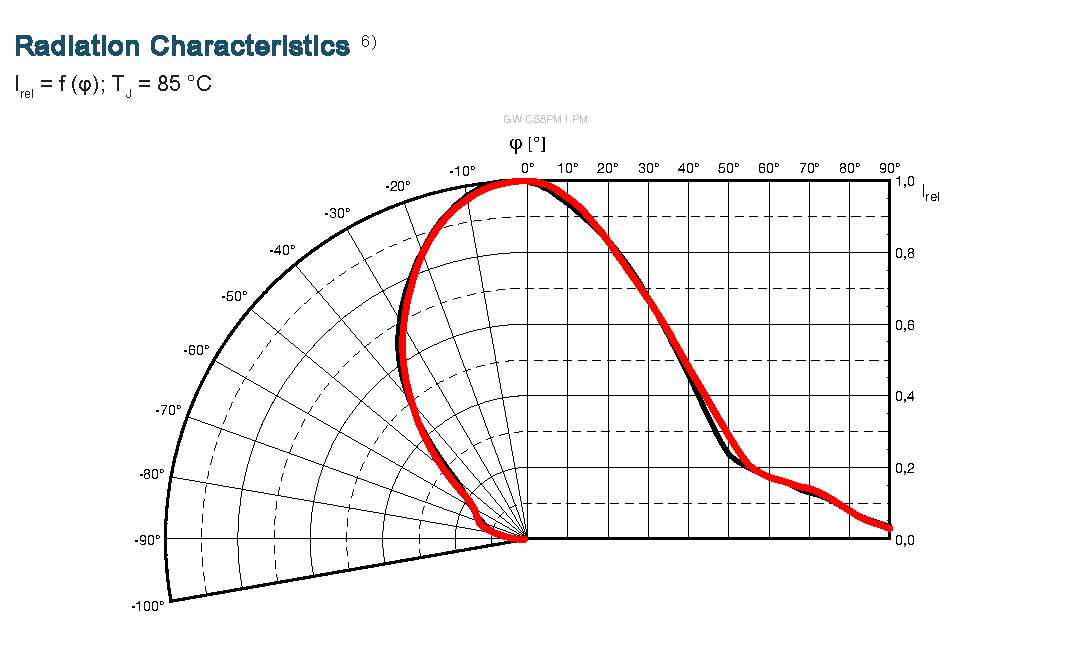
\includegraphics[width=0.61\linewidth]{assets/led-ds-radiacion.pdf}}
\caption*{\footnotesize\raggedright Figura 8 — Diagrama de radiación. La intensidad relativa cae a 0,5 cerca de $\pm$40\textdegree{} y conserva valores apreciables hasta $\pm$70\textdegree{}. {\color{gray2}Fuente: ams OSRAM, datasheet GW CS8PM1.PM, versión 1.10, 2026-03-05, p. 12.}}
\end{figure}

\subsection*{5. Alimentación y driver recomendado}
\addcontentsline{toc}{subsection}{5. Alimentación y driver recomendado}

El LED se alimenta con \textbf{corriente constante, nunca con tensión fija}. Su tensión directa varía entre unidades (2,70–3,20 V) y baja con la temperatura; con una fuente de tensión, pequeñas diferencias de Vf se traducen en grandes diferencias de corriente y la unidad puede entrar en embalamiento térmico.

\begingroup\footnotesize
\setlength{\tabcolsep}{4pt}
\setlength{\emergencystretch}{4em}
\hyphenpenalty=50 \exhyphenpenalty=50
\begin{longtable}{@{}>{\RaggedRight\arraybackslash}p{\dimexpr 0.2053\linewidth-2\tabcolsep\relax}>{\RaggedRight\arraybackslash}p{\dimexpr 0.3948\linewidth-2\tabcolsep\relax}>{\RaggedRight\arraybackslash}p{\dimexpr 0.3948\linewidth-2\tabcolsep\relax}@{}}
\toprule
\scriptsize\textbf{Parámetro del driver} & \scriptsize\textbf{Recomendación} & \scriptsize\textbf{Justificación} \\
\midrule
\endfirsthead
\toprule
\scriptsize\textbf{Parámetro del driver} & \scriptsize\textbf{Recomendación} & \scriptsize\textbf{Justificación} \\
\midrule
\endhead
\bottomrule
\endfoot
Tipo & Fuente de corriente constante, preferentemente conmutada (\emph{buck}) & Regula corriente con independencia del Vf de cada unidad \\
Corriente nominal & \textbf{350 mA} & Punto en que el datasheet especifica flujo, Vf y CRI \\
Tensión de \emph{compliance} & $\geq$ 3,5 V en el LED más el margen propio del driver & Vf máx. 3,20 V a 85 \textdegree{}C, más $\approx$ 0,3 V de aumento a $-$40 \textdegree{}C según la curva $\Delta$Vf(Tj) \\
Alimentación de entrada & Bus de 12 V o 24 V del robot & Con un regulador lineal desde 5 V se disiparían $\approx$ 0,75 W en el regulador \\
Regulación de brillo & PWM sobre la entrada \emph{enable}, con pulso de 350 mA & El datasheet prohíbe operar en continua por debajo de 100 mA \\
Frecuencia PWM & Alta frente al tiempo de exposición, o sincronizada con la cámara & Evita bandas y variaciones de brillo entre cuadros \\
Protecciones & Circuito abierto, cortocircuito y reducción de corriente por temperatura (NTC cerca del LED) & Operación 24/7 sin supervisión \\
\end{longtable}
\endgroup

\begin{figure}[htbp]\centering
\fbox{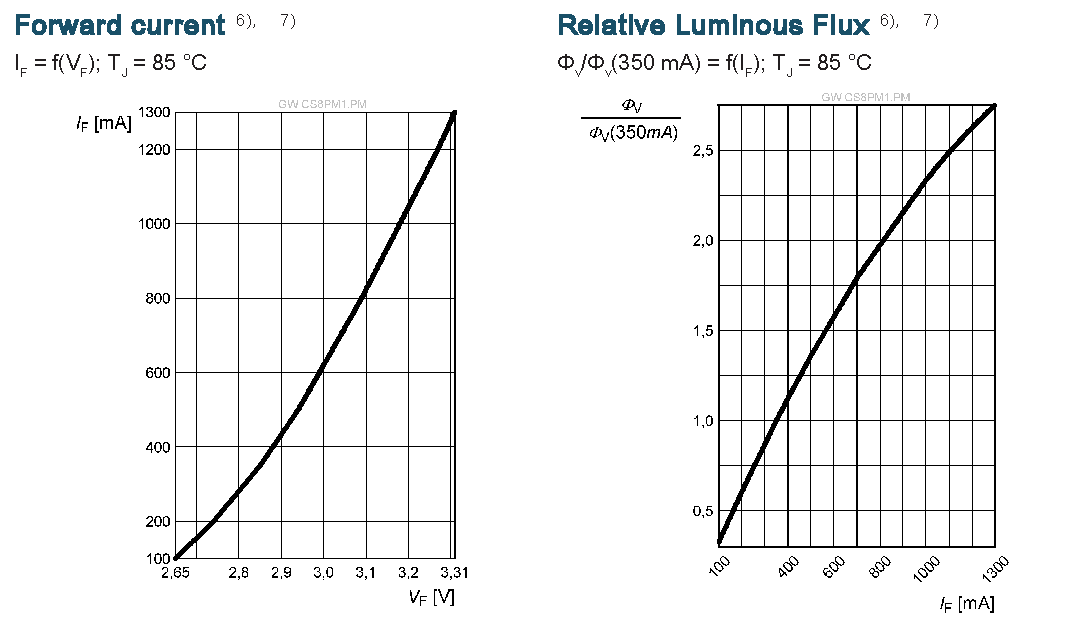
\includegraphics[width=0.98\linewidth]{assets/led-ds-corriente.pdf}}
\caption*{\footnotesize\raggedright Figura 9 — Corriente frente a tensión directa y flujo relativo frente a corriente a Tj = 85 \textdegree{}C. A 500 mA el flujo sube $\approx$ 36 \% respecto de 350 mA; a 700 mA, $\approx$ 80 \%. {\color{gray2}Fuente: ams OSRAM, datasheet GW CS8PM1.PM, versión 1.10, 2026-03-05, p. 13.}}
\end{figure}

\subsubsection*{Confiabilidad y diseño térmico}
\addcontentsline{toc}{subsubsection}{Confiabilidad y diseño térmico}

Con RthJS = 3,7 K/W y 1,0 W eléctrico, la juntura queda apenas \textbf{$\approx$ 4 K por encima del punto de soldadura}. Por eso, en este diseño, el cuello de botella térmico \textbf{no es el LED}: es la trayectoria del calor desde la placa hacia el cuerpo de aluminio.

\begin{itemize}
\item Usar placa \textbf{MCPCB} o PCB con vías térmicas bajo el \emph{pad} central, que según el plano no tiene conexión eléctrica, y acoplarla al cuerpo de aluminio con interfaz térmica.
\item Medir la temperatura en el punto de soldadura, o lo más cerca posible del LED, durante un ensayo 24/7 en la peor condición ambiente.
\item Mantener la juntura con margen amplio respecto de 135 \textdegree{}C. Como referencia de diseño, conviene no superar $\approx$ 85 \textdegree{}C de Ts en régimen, que es además la temperatura a la que el datasheet especifica el flujo.
\item La curva de derating permite 1300 mA hasta Ts = 100 \textdegree{}C. Si se sube la corriente para recuperar flujo, hay que recalcular disipación, derating y vida útil, y confirmar la temperatura con medición.
\end{itemize}

\begin{figure}[htbp]\centering
\fbox{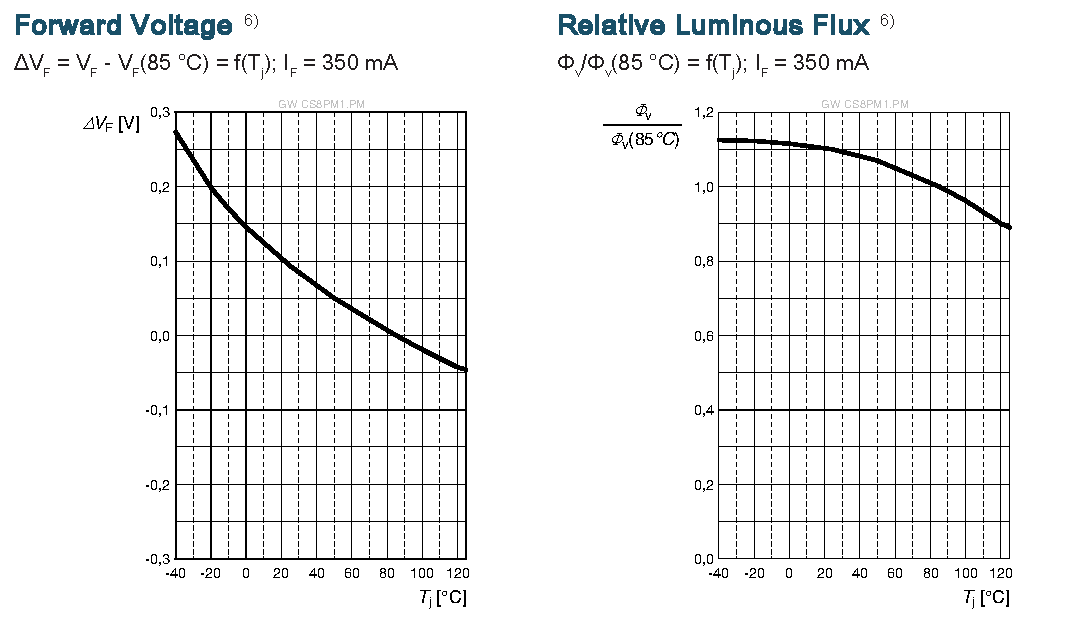
\includegraphics[width=0.98\linewidth]{assets/led-ds-temperatura.pdf}}
\caption*{\footnotesize\raggedright Figura 10 — Variación de Vf y de flujo relativo con la temperatura de juntura a 350 mA. El flujo a 25 \textdegree{}C es $\approx$ 10 \% mayor que a 85 \textdegree{}C, y a 120 \textdegree{}C cae $\approx$ 10 \%. {\color{gray2}Fuente: ams OSRAM, datasheet GW CS8PM1.PM, versión 1.10, 2026-03-05, p. 14.}}
\end{figure}
\begin{figure}[htbp]\centering
\fbox{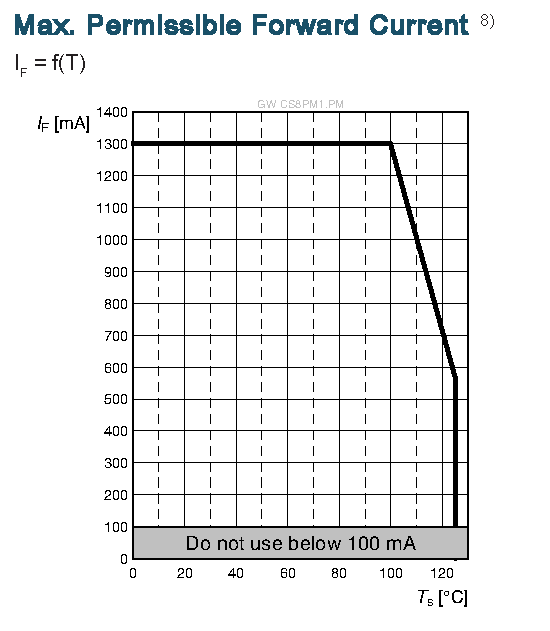
\includegraphics[width=0.49\linewidth]{assets/led-ds-derating.pdf}}
\caption*{\footnotesize\raggedright Figura 11 — Corriente máxima admisible frente a la temperatura del punto de soldadura. Plena corriente hasta Ts = 100 \textdegree{}C y prohibición de operar por debajo de 100 mA. {\color{gray2}Fuente: ams OSRAM, datasheet GW CS8PM1.PM, versión 1.10, 2026-03-05, p. 15.}}
\end{figure}
\clearpage

\section*{Parte III — Cálculo óptico}
\addcontentsline{toc}{section}{Parte III — Cálculo óptico}


\subsection*{6. Geometría y captura directa}
\addcontentsline{toc}{subsection}{6. Geometría y captura directa}

La ventana tiene radio r = 2,5 mm y está a d = 7 mm del emisor. El semiángulo que la ventana subtiende desde el LED es:

\begin{itemize}
\item \texttt{$\alpha$ = atan(r / d) = atan(2,5 / 7) = 19,65\textdegree{}}
\end{itemize}

Para la distribución angular del LED se usa el modelo habitual \texttt{I($\theta$) = I0 \textperiodcentered{} cos\textasciicircum{}m($\theta$)}. Como la intensidad cae al 50 \% a 40\textdegree{}:

\begin{itemize}
\item \texttt{m = ln(0,5) / ln(cos 40\textdegree{}) = 2,60}
\end{itemize}

La fracción del flujo total que sale dentro de un semiángulo $\alpha$ es \texttt{F($\alpha$) = 1 $-$ cos\textasciicircum{}(m+1)($\alpha$)}. Para la ventana:

\begin{itemize}
\item \texttt{F\_directa = 1 $-$ cos(19,65\textdegree{})\textasciicircum{}3,60 $\approx$ 0,194}
\end{itemize}

\begingroup\footnotesize
\setlength{\tabcolsep}{4pt}
\setlength{\emergencystretch}{4em}
\hyphenpenalty=50 \exhyphenpenalty=50
\begin{longtable}{@{}>{\RaggedRight\arraybackslash}p{\dimexpr 0.4178\linewidth-2\tabcolsep\relax}>{\RaggedRight\arraybackslash}p{\dimexpr 0.5772\linewidth-2\tabcolsep\relax}@{}}
\toprule
\scriptsize\textbf{Flujo del LED (bin LUMQ)} & \scriptsize\textbf{Luz directa en la ventana, antes del difusor} \\
\midrule
\endfirsthead
\toprule
\scriptsize\textbf{Flujo del LED (bin LUMQ)} & \scriptsize\textbf{Luz directa en la ventana, antes del difusor} \\
\midrule
\endhead
\bottomrule
\endfoot
164 lm (mínimo del bin) & \textbf{32 lm} \\
187 lm (valor medio, usado en los cálculos) & \textbf{36 lm} \\
210 lm (máximo del bin) & \textbf{41 lm} \\
\end{longtable}
\endgroup

\begin{notaclave}{Conclusión parcial}
Sin recuperación de luz por reflexiones en el conducto, \textbf{no se llega a 100 lm}. Cuatro de cada cinco lúmenes del LED tocan la pared antes de poder llegar a la ventana, así que la eficiencia real depende de cuánto recupere el conducto de aluminio.

\end{notaclave}

\subsection*{7. Conducto de aluminio fresado: dos escenarios}
\addcontentsline{toc}{subsection}{7. Conducto de aluminio fresado: dos escenarios}

El conducto se trata como una \textbf{guía óptica imperfecta}. Como su reflectividad y su especularidad no se conocen, se calculan dos escenarios que acotan el comportamiento real, cada uno con una reflectividad de pared entre 0,55 y 0,92.

El cálculo es una simulación Monte Carlo simplificada, reproducible con \texttt{tools/led\_montecarlo.py}: fuente puntual con distribución cos\textasciicircum{}2,6 en el fondo de un cilindro de Ø 5 $\times$ 7 mm, fondo absorbente y toda la boca como ventana. Con 400.000 rayos, reproduce las tablas de partida con diferencias menores a 0,01 en eficiencia.


\subsubsection*{Modelo conservador: pared difusa}
\addcontentsline{toc}{subsubsection}{Modelo conservador: pared difusa}

Aluminio mecanizado sin pulir que refleja de manera mayormente difusa: cada rebote reparte la luz en todas direcciones, y parte vuelve hacia el fondo.

\begingroup\footnotesize
\setlength{\tabcolsep}{3pt}
\setlength{\emergencystretch}{4em}
\hyphenpenalty=50 \exhyphenpenalty=50
\begin{longtable}{@{}>{\RaggedRight\arraybackslash}p{\dimexpr 0.2349\linewidth-2\tabcolsep\relax}>{\RaggedRight\arraybackslash}p{\dimexpr 0.2158\linewidth-2\tabcolsep\relax}>{\RaggedRight\arraybackslash}p{\dimexpr 0.2440\linewidth-2\tabcolsep\relax}>{\RaggedRight\arraybackslash}p{\dimexpr 0.1501\linewidth-2\tabcolsep\relax}>{\RaggedRight\arraybackslash}p{\dimexpr 0.1501\linewidth-2\tabcolsep\relax}@{}}
\toprule
\scriptsize\textbf{Reflectividad de la pared} & \scriptsize\textbf{Eficiencia del conducto} & \scriptsize\textbf{Antes del difusor (187 lm)} & \scriptsize\textbf{Con difusor 75 \%} & \scriptsize\textbf{Con difusor 90 \%} \\
\midrule
\endfirsthead
\toprule
\scriptsize\textbf{Reflectividad de la pared} & \scriptsize\textbf{Eficiencia del conducto} & \scriptsize\textbf{Antes del difusor (187 lm)} & \scriptsize\textbf{Con difusor 75 \%} & \scriptsize\textbf{Con difusor 90 \%} \\
\midrule
\endhead
\bottomrule
\endfoot
0,55 & 0,29 & 55 lm & 41 lm & 49 lm \\
0,65 & 0,33 & 62 lm & 46 lm & 56 lm \\
0,75 & 0,37 & 70 lm & 52 lm & 63 lm \\
0,85 & 0,44 & 82 lm & 62 lm & 74 lm \\
0,92 & 0,50 & 93 lm & 70 lm & 83 lm \\
\end{longtable}
\endgroup


\subsubsection*{Modelo optimista: pared con componente especular apreciable}
\addcontentsline{toc}{subsubsection}{Modelo optimista: pared con componente especular apreciable}

Aluminio limpio, con marcas de herramienta finas pero sin pulir, que conserva buena parte de la reflexión especular. El conducto funciona entonces como una guía de luz y conserva la componente axial.

\begingroup\footnotesize
\setlength{\tabcolsep}{3pt}
\setlength{\emergencystretch}{4em}
\hyphenpenalty=50 \exhyphenpenalty=50
\begin{longtable}{@{}>{\RaggedRight\arraybackslash}p{\dimexpr 0.2349\linewidth-2\tabcolsep\relax}>{\RaggedRight\arraybackslash}p{\dimexpr 0.2158\linewidth-2\tabcolsep\relax}>{\RaggedRight\arraybackslash}p{\dimexpr 0.2440\linewidth-2\tabcolsep\relax}>{\RaggedRight\arraybackslash}p{\dimexpr 0.1501\linewidth-2\tabcolsep\relax}>{\RaggedRight\arraybackslash}p{\dimexpr 0.1501\linewidth-2\tabcolsep\relax}@{}}
\toprule
\scriptsize\textbf{Reflectividad de la pared} & \scriptsize\textbf{Eficiencia del conducto} & \scriptsize\textbf{Antes del difusor (187 lm)} & \scriptsize\textbf{Con difusor 75 \%} & \scriptsize\textbf{Con difusor 90 \%} \\
\midrule
\endfirsthead
\toprule
\scriptsize\textbf{Reflectividad de la pared} & \scriptsize\textbf{Eficiencia del conducto} & \scriptsize\textbf{Antes del difusor (187 lm)} & \scriptsize\textbf{Con difusor 75 \%} & \scriptsize\textbf{Con difusor 90 \%} \\
\midrule
\endhead
\bottomrule
\endfoot
0,55 & 0,56 & 105 lm & 79 lm & 95 lm \\
0,65 & 0,65 & 121 lm & 90 lm & 109 lm \\
0,75 & 0,74 & 138 lm & 103 lm & 124 lm \\
0,85 & 0,83 & 156 lm & 117 lm & 140 lm \\
0,92 & 0,91 & 170 lm & 127 lm & 153 lm \\
\end{longtable}
\endgroup

\begin{figure}[htbp]\centering
\fbox{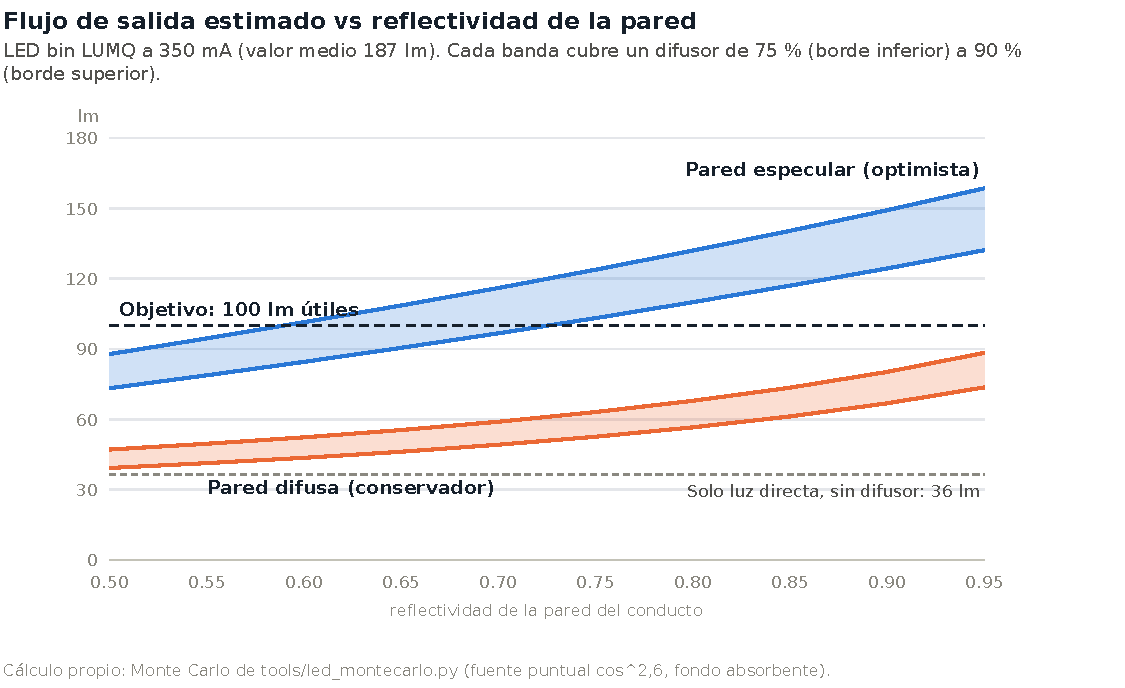
\includegraphics[width=0.88\linewidth]{assets/led-sensibilidad.pdf}}
\caption*{\footnotesize\raggedright Figura 12 — Flujo de salida estimado en función de la reflectividad de la pared, para los dos modelos. El ancho de cada banda es el efecto del difusor (75 \% a 90 \%). {\color{gray2}Cálculo propio con tools/led\_montecarlo.py.}}
\end{figure}

\subsection*{8. Rango estimado de flujo real y condiciones para 100 lm}
\addcontentsline{toc}{subsection}{8. Rango estimado de flujo real y condiciones para 100 lm}

Para entregar 100 lm con el valor medio del bin (187 lm), el conjunto conducto + difusor debe tener una eficiencia de al menos \textbf{0,54}. Eso exige una eficiencia de conducto de \textbf{0,59 con difusor de 90 \%} o de \textbf{0,71 con difusor de 75 \%}.

\begingroup\footnotesize
\setlength{\tabcolsep}{4pt}
\setlength{\emergencystretch}{4em}
\hyphenpenalty=50 \exhyphenpenalty=50
\begin{longtable}{@{}>{\RaggedRight\arraybackslash}p{\dimexpr 0.4648\linewidth-2\tabcolsep\relax}>{\RaggedRight\arraybackslash}p{\dimexpr 0.3570\linewidth-2\tabcolsep\relax}>{\RaggedRight\arraybackslash}p{\dimexpr 0.1731\linewidth-2\tabcolsep\relax}@{}}
\toprule
\scriptsize\textbf{Situación} & \scriptsize\textbf{Flujo de salida probable a 350 mA} & \scriptsize\textbf{¿Llega a 100 lm?} \\
\midrule
\endfirsthead
\toprule
\scriptsize\textbf{Situación} & \scriptsize\textbf{Flujo de salida probable a 350 mA} & \scriptsize\textbf{¿Llega a 100 lm?} \\
\midrule
\endhead
\bottomrule
\endfoot
Pared mate o difusa, difusor 75–90 \% & 40–80 lm & No \\
Pared con componente especular, Rw $\geq$ 0,60, difusor 90 \% & 100–155 lm & Sí \\
Pared con componente especular, Rw $\geq$ 0,73, difusor 75 \% & 100–127 lm & Sí, con poco margen \\
Bin mínimo (164 lm), pared especular Rw 0,75, difusor 85 \% & $\approx$ 103 lm & Justo \\
\end{longtable}
\endgroup

\begin{notainferencia}{Conclusión óptica}
\begin{itemize}
\item El objetivo de \textbf{100 lm a la salida es viable} si el conducto conserva una componente especular razonable y el difusor tiene transmisión alta.
\item Con pared muy mate o difusa, el flujo probable cae a \textbf{40–80 lm} a 350 mA, aun con el bin LUMQ.
\item Un aluminio fresado real queda \textbf{entre los dos modelos}, y dónde queda solo lo dice una medición.
\end{itemize}

\end{notainferencia}
Para \textbf{garantizar} los 100 lm hay tres palancas, en orden de preferencia:

\begin{enumerate}
\item \textbf{Mejorar la pared}: pulido del conducto, inserto de aluminio reflectivo o film especular, recubrimiento blanco de alta reflectancia (\textgreater{} 0,95) o reflector metalizado. Es la palanca más efectiva, porque actúa sobre el 80 \% del flujo que hoy depende de la pared.
\item \textbf{Difusor de alta transmisión}, 85–90 \%, con la difusión justa para homogeneizar el punto caliente.
\item \textbf{Subir la corriente} solo si el diseño térmico lo permite. A 500 mA el flujo sube $\approx$ 36 \% (Figura 9) con $\approx$ 1,5 W eléctricos. Por ejemplo, pared difusa de 0,85 con difusor de 90 \% pasa de 74 lm a $\approx$ 100 lm.
\end{enumerate}

También puede \textbf{revisarse la geometría}: acortar la distancia LED–ventana o ensanchar la ventana aumenta $\alpha$, y con él la captura directa.

\clearpage

\section*{Parte IV — Riesgos, industrialización y abastecimiento}
\addcontentsline{toc}{section}{Parte IV — Riesgos, industrialización y abastecimiento}


\subsection*{9. Riesgos}
\addcontentsline{toc}{subsection}{9. Riesgos}

\begingroup\footnotesize
\setlength{\tabcolsep}{4pt}
\setlength{\emergencystretch}{4em}
\hyphenpenalty=50 \exhyphenpenalty=50
\begin{longtable}{@{}>{\RaggedRight\arraybackslash}p{\dimexpr 0.3088\linewidth-2\tabcolsep\relax}>{\RaggedRight\arraybackslash}p{\dimexpr 0.3431\linewidth-2\tabcolsep\relax}>{\RaggedRight\arraybackslash}p{\dimexpr 0.3431\linewidth-2\tabcolsep\relax}@{}}
\toprule
\scriptsize\textbf{Riesgo} & \scriptsize\textbf{Efecto} & \scriptsize\textbf{Mitigación} \\
\midrule
\endfirsthead
\toprule
\scriptsize\textbf{Riesgo} & \scriptsize\textbf{Efecto} & \scriptsize\textbf{Mitigación} \\
\midrule
\endhead
\bottomrule
\endfoot
Reflectividad incierta del aluminio fresado & Salida entre 40 y 140 lm según la pared & Medir sobre prototipo; tener definido un tratamiento de pared como plan B \\
Dispersión del bin (164–210 lm) & $\pm$12 \% sobre el valor medio & Diseñar con 164 lm; especificar el bin LUMQ en la orden de compra \\
Condición de medición del bin & La portada indica 155 lm típicos a 85 \textdegree{}C, mientras el bin se mide con pulso de 10 ms. Si el bin estuviera referido a 25 \textdegree{}C, en régimen el flujo sería $\approx$ 10 \% menor & Confirmar con ams OSRAM la temperatura de referencia del bin; medir flujo en régimen térmico estable \\
Temperatura & $\approx$ $-$10 \% de flujo a 120 \textdegree{}C de juntura respecto de 85 \textdegree{}C; degradación más rápida & Trayectoria térmica a la carcasa, NTC y reducción de corriente \\
Envejecimiento y contaminación de la lente de silicona & Pérdida de flujo y corrimiento de color & Evitar compuestos volátiles (adhesivos y juntas no compatibles) dentro del conducto cerrado \\
Materiales con plata en el LED & Decoloración ante atmósferas con azufre o agentes agresivos & Revisar compatibilidad con los productos de limpieza de la farmacia; sellar el módulo \\
CRI 70 & Reproducción de color limitada; R9 puede ser $-$40 & Suficiente para forma, presencia, bordes, contraste y lectura. Para medir color con precisión, evaluar una variante de CRI 80–90 \\
Deslumbramiento & Clasificación IEC 62471 de riesgo moderado (tiempo de exposición de 0,25 s) & El difusor reduce la luminancia; evitar la visión directa durante el mantenimiento \\
Aplicación médica o de seguridad & El fabricante no califica el componente para estos usos & Ver la nota siguiente \\
Disponibilidad y obsolescencia de subvariantes & El datasheet cambió la tabla de pedido en 2025 y 2026 & Aprobar XX53 y A333 como alternativas; evitar bins antiguos como LSLU \\
\end{longtable}
\endgroup

\begin{notariesgo}{Advertencia regulatoria}
El datasheet indica que estos componentes \textbf{no están desarrollados, construidos ni ensayados como componente de seguridad ni para dispositivos médicos}, y que no están calificados a nivel de módulo ni de sistema para esos usos. En el robot de farmacia el LED es válido como \textbf{componente de iluminación}. Si su función afecta la seguridad o la dispensación, por ejemplo cuando una cámara verifica el medicamento dispensado, el sistema completo debe evaluarse según la normativa aplicable, y el fabricante pide que se le informe ese uso.

\end{notariesgo}

\subsection*{10. Calidad, robustez e industrialización}
\addcontentsline{toc}{subsection}{10. Calidad, robustez e industrialización}

\begin{itemize}
\item Familia industrial de ams OSRAM, orientada a iluminación profesional, interior, exterior e industrial.
\item Paquete cerámico con lente de silicona y baja resistencia térmica, una ventaja frente a LEDs plásticos de bajo costo.
\item Compatible con montaje SMD automático: cinta y carrete de 600 unidades, MSL 2 y perfil de reflow sin plomo estándar. El fabricante recomienda soldar en atmósfera de nitrógeno.
\item Apto para funcionamiento 24/7 siempre que el driver sea de corriente constante, haya disipación real hacia el cuerpo de aluminio, la juntura opere con margen y la lente no se contamine químicamente.
\end{itemize}

\begin{figure}[htbp]\centering
\fbox{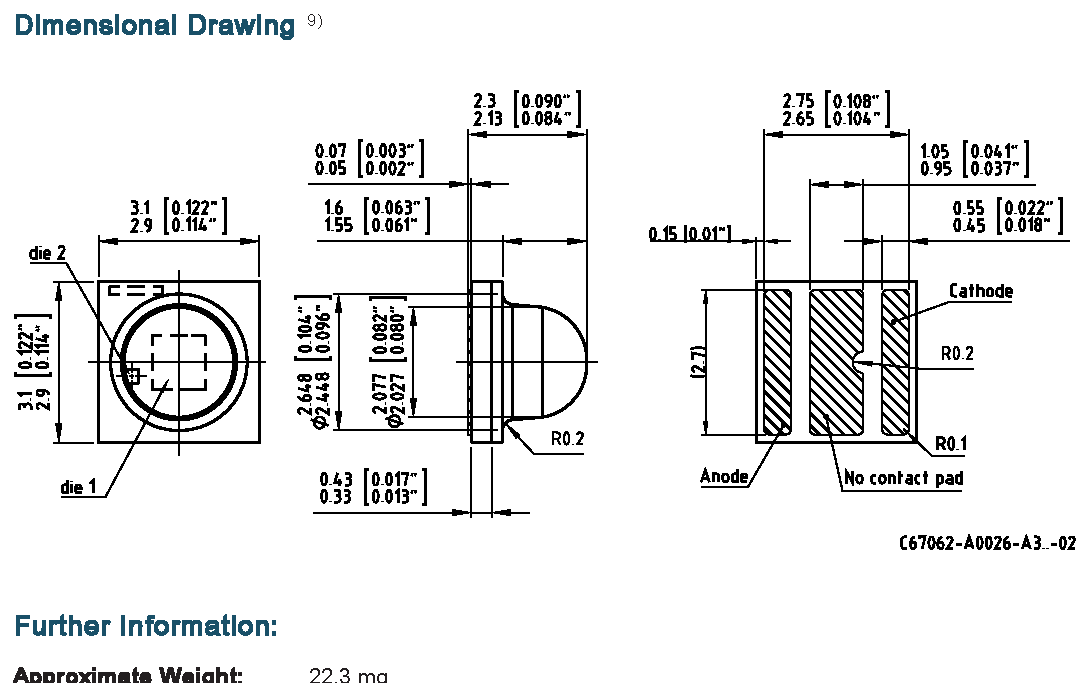
\includegraphics[width=0.98\linewidth]{assets/led-ds-dimensiones.pdf}}
\caption*{\footnotesize\raggedright Figura 13 — Plano dimensional: cuerpo de 2,9–3,1 mm, altura de 2,13–2,30 mm, ánodo, cátodo y pad central sin conexión eléctrica. {\color{gray2}Fuente: ams OSRAM, datasheet GW CS8PM1.PM, versión 1.10, 2026-03-05, p. 16.}}
\end{figure}
\begin{figure}[htbp]\centering
\fbox{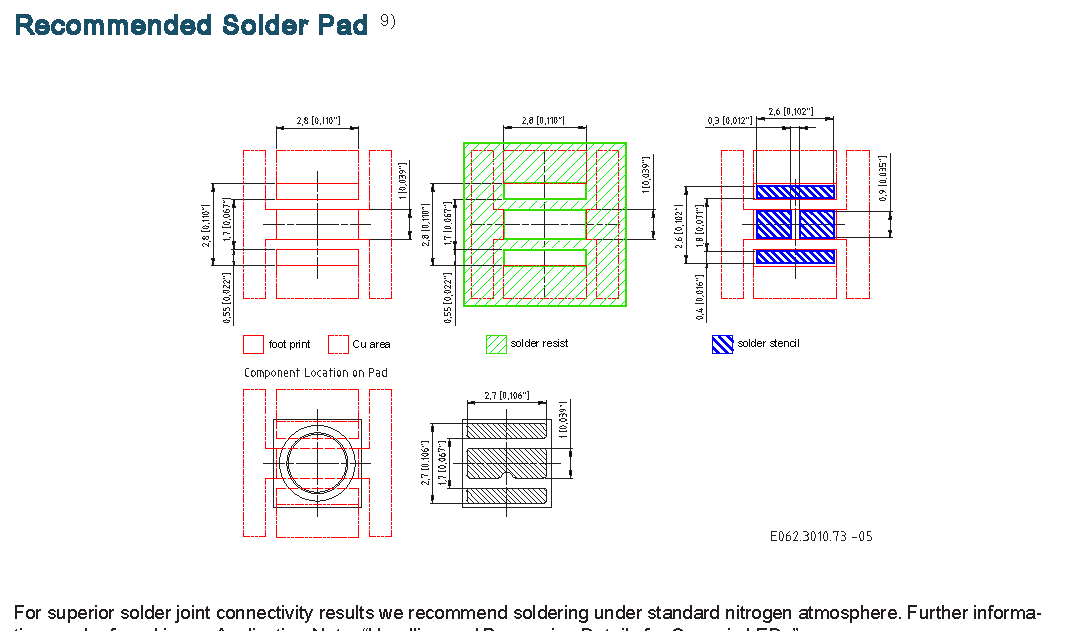
\includegraphics[width=0.98\linewidth]{assets/led-ds-footprint.pdf}}
\caption*{\footnotesize\raggedright Figura 14 — Pads de soldadura recomendados. {\color{gray2}Fuente: ams OSRAM, datasheet GW CS8PM1.PM, versión 1.10, 2026-03-05, p. 17.}}
\end{figure}
\begin{figure}[htbp]\centering
\fbox{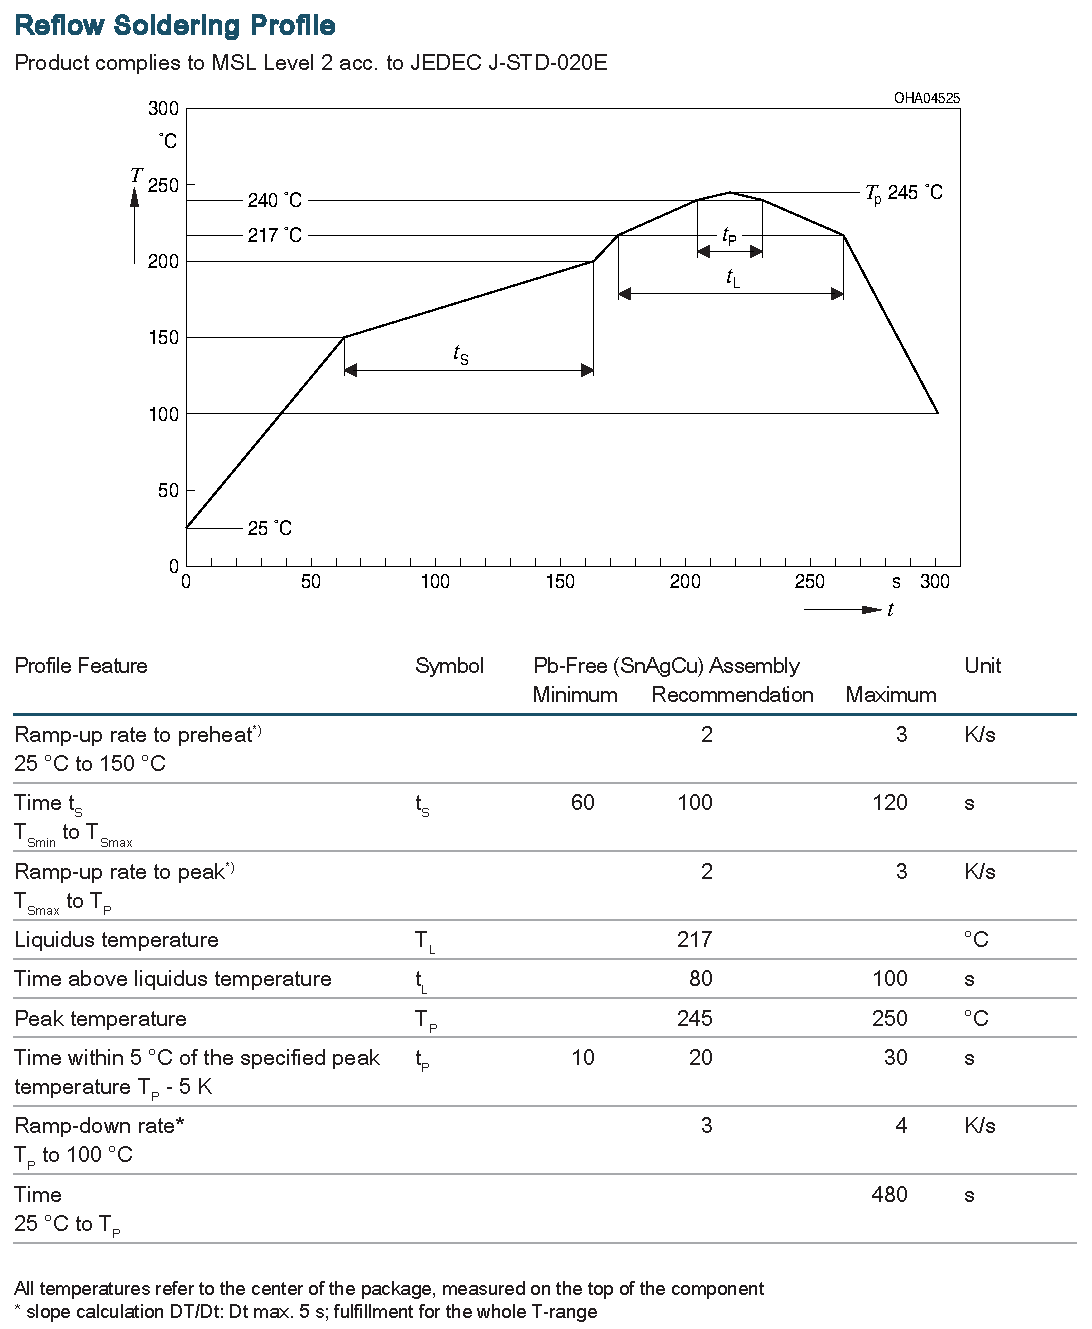
\includegraphics[width=0.76\linewidth]{assets/led-ds-reflow.pdf}}
\caption*{\footnotesize\raggedright Figura 15 — Perfil de reflow sin plomo: pico de 245 \textdegree{}C recomendado y 250 \textdegree{}C máximo; MSL 2 según JEDEC J-STD-020E. {\color{gray2}Fuente: ams OSRAM, datasheet GW CS8PM1.PM, versión 1.10, 2026-03-05, p. 18.}}
\end{figure}

\subsection*{11. Precio, stock y disponibilidad}
\addcontentsline{toc}{subsection}{11. Precio, stock y disponibilidad}

Relevamiento del 27 de septiembre de 2026. Precios sin impuestos ni envío.

\begingroup\footnotesize
\setlength{\tabcolsep}{3pt}
\setlength{\emergencystretch}{4em}
\hyphenpenalty=50 \exhyphenpenalty=50
\begin{longtable}{@{}>{\RaggedRight\arraybackslash}p{\dimexpr 0.1069\linewidth-2\tabcolsep\relax}>{\RaggedRight\arraybackslash}p{\dimexpr 0.2467\linewidth-2\tabcolsep\relax}>{\RaggedRight\arraybackslash}p{\dimexpr 0.1932\linewidth-2\tabcolsep\relax}>{\RaggedRight\arraybackslash}p{\dimexpr 0.2467\linewidth-2\tabcolsep\relax}>{\RaggedRight\arraybackslash}p{\dimexpr 0.2015\linewidth-2\tabcolsep\relax}@{}}
\toprule
\scriptsize\textbf{Fuente} & \scriptsize\textbf{Parte} & \scriptsize\textbf{Estado \slash  stock} & \scriptsize\textbf{Precio observado} & \scriptsize\textbf{Comentario} \\
\midrule
\endfirsthead
\toprule
\scriptsize\textbf{Fuente} & \scriptsize\textbf{Parte} & \scriptsize\textbf{Estado \slash  stock} & \scriptsize\textbf{Precio observado} & \scriptsize\textbf{Comentario} \\
\midrule
\endhead
\bottomrule
\endfoot
ams OSRAM oficial & GW CS8PM1.PM-LUMQ-A333-1 / XX53-1 & Producción plena & No publica precio & Fuente técnica primaria \\
Mouser Europa (Alemania) & GW CS8PM1.PM-LUMQ-XX53-1-350-R18 & 1.669 unidades & 1 u.: 1,33 EUR \textperiodcentered{} 10: 0,937 EUR \textperiodcentered{} 100: 0,698 EUR \textperiodcentered{} carrete 600: 0,593 EUR & Referencia de costo real para compra baja y media \\
Mouser Brasil & GW CS8PM1.PM-LUMQ-XX53-1-350-R18 & 1.669 unidades & 1 u.: USD 1,55 \textperiodcentered{} 100: USD 0,812 \textperiodcentered{} carrete 600: USD 0,689 & Referencia regional \\
DigiKey & GW CS8PM1.PM-LUMQ-XX53-1-350-R18 & Activo, sin stock habitual; requiere cotización & Sin precio directo & Confirma parámetros eléctricos y mecánicos \\
Mouser Argentina & Variantes OSLON SSL 80 relacionadas & Variante LTMP 6500 K sin stock, mínimo 600 & ARS 1.128,58 c/u a 600 (variante relacionada) & No confirma disponibilidad local del LUMQ 5000 K \\
TME Argentina & Categoría LEDs blancos de potencia ams OSRAM & Verificar parte exacta & No confirmado & Posible canal alternativo \\
\end{longtable}
\endgroup

\begin{notaclave}{Conclusiones de compra}
\begin{itemize}
\item Comprar la variante objetivo \textbf{LUMQ 5000 K} (XX53-1, o A333-1 como alternativa aprobada).
\item No comprar variantes viejas u obsoletas como \textbf{LSLU}, salvo para prototipo o aceptando menor flujo.
\item En Argentina es más realista \textbf{importar por Mouser, DigiKey o TME} que esperar stock local de la parte exacta.
\item Confirmar pedido mínimo, carrete de 600 y plazos de entrega antes de congelar la lista de materiales.
\item Costo del LED en volumen de carrete: \textbf{$\approx$ 0,60 EUR por unidad}, irrelevante frente al costo del módulo.
\end{itemize}

\end{notaclave}
\clearpage

\section*{Parte V — Validación}
\addcontentsline{toc}{section}{Parte V — Validación}


\subsection*{12. Recomendaciones de prototipo}
\addcontentsline{toc}{subsection}{12. Recomendaciones de prototipo}

\begin{enumerate}
\item \textbf{Medir el flujo real de salida} con esfera integradora o con un sensor calibrado, en régimen térmico estable a 350 mA. Es la medición que cierra la incógnita de este informe.
\item \textbf{Medir temperatura} en el punto de soldadura, o cerca del LED, durante un ensayo 24/7 a la máxima temperatura ambiente prevista.
\item \textbf{Comparar conductos}: mecanizado tal como sale de máquina, pulido, con inserto o film reflectivo y con recubrimiento blanco de alta reflectancia. Con los resultados se ajusta el modelo de la sección 7.
\item \textbf{Evaluar difusores} de transmisión conocida (75 \%, 85 \% y 90 \%) y medir la uniformidad del punto de luz junto con el flujo.
\item \textbf{Validar con la cámara o el sensor real} del robot: contraste, uniformidad, ausencia de parpadeo con el PWM elegido y estabilidad del color en el tiempo.
\item \textbf{Verificar tolerancias}: centrado del LED en el conducto y distancia real LED–ventana, incluida la altura del encapsulado de 2,13–2,30 mm.
\end{enumerate}

\begin{detalle}{Criterio de aceptación sugerido para el prototipo}
\begin{itemize}
\item Flujo de salida $\geq$ 100 lm medido con un LED de bin LUMQ a 350 mA, en régimen térmico estable.
\item Ts $\leq$ 85 \textdegree{}C en la peor condición ambiente, con ensayo continuo de al menos 72 h.
\item Uniformidad y contraste aceptados por el equipo de visión artificial.
\item Sin decoloración visible de la lente tras la exposición a los agentes de limpieza previstos.
\end{itemize}

\end{detalle}
\clearpage

\section*{Anexos}
\addcontentsline{toc}{section}{Anexos}


\subsection*{Anexo A — Fuentes verificadas}
\addcontentsline{toc}{subsection}{Anexo A — Fuentes verificadas}

\begin{itemize}
\item ams OSRAM, página de producto OSRAM OSLON SSL 80 GW CS8PM1.PM: \url{https://ams-osram.com/products/leds/white-leds/osram-oslon-ssl-80-gw-cs8pm1-pm}
\item ams OSRAM, datasheet oficial GW CS8PM1.PM, versión 1.10, 2026-03-05: \url{https://look.ams-osram.com/m/16996c4989af2a7d/original/GW-CS8PM1-PM.pdf}
\item Mouser Europa, GW CS8PM1.PM-LUMQ-XX53-1-350-R18: \url{https://www.mouser.de/ProductDetail/ams-OSRAM/GW-CS8PM1.PM-LUMQ-XX53-1-350-R18}
\item Mouser Brasil, GW CS8PM1.PM-LUMQ-XX53-1-350-R18: \url{https://br.mouser.com/ProductDetail/ams-OSRAM/GW-CS8PM1.PM-LUMQ-XX53-1-350-R18}
\item DigiKey, GW CS8PM1.PM-LUMQ-XX53-1-350-R18: \url{https://www.digikey.com/en/products/detail/ams-osram-ag/GW-CS8PM1-PM-LUMQ-XX53-1-350-R18/26248732}
\item Mouser Argentina, variante relacionada OSLON SSL 80: \url{https://ar.mouser.com/ProductDetail/ams-OSRAM/GW-CS8PM1.PMLTMPXX51}
\item TME Argentina, categoría LEDs de potencia blancos ams OSRAM: \url{https://www.tme.com/ar/es/katalog/leds-de-potencia-blancos_113364/p%2Cams-osram_114/}
\end{itemize}

\begin{notadato}{Alcance de la verificación}
Los datos técnicos de este informe se contrastaron con el datasheet oficial v1.10: pedido, valores máximos, características, grupos, curvas, plano, reflow, notas y descargo. Los precios y el stock de distribuidores provienen del relevamiento del 27-09-2026 y pueden cambiar en días. Las cifras de flujo de salida son cálculos propios con los supuestos declarados en la sección 7.

\end{notadato}

\subsection*{Anexo B — Método de cálculo}
\addcontentsline{toc}{subsection}{Anexo B — Método de cálculo}

\begin{itemize}
\item \textbf{Modelo angular del LED}: \texttt{I($\theta$) = I0\textperiodcentered{}cos\textasciicircum{}m($\theta$)}, con m = 2,60 para 2$\varphi$ = 80\textdegree{}. Para los LEDs de comparación, m = 1,00 (120\textdegree{}, lambertiano) y m = 0,51 (150\textdegree{}).
\item \textbf{Captura directa}: \texttt{F($\alpha$) = 1 $-$ cos\textasciicircum{}(m+1)($\alpha$)}, con $\alpha$ = 19,65\textdegree{}.
\item \textbf{Conducto}: trazado de rayos Monte Carlo en un cilindro de Ø 5 $\times$ 7 mm con fuente puntual en el centro del fondo. La pared es difusa (lambertiana) o especular ideal, con reflectividad Rw por rebote; el fondo es absorbente y la salida es la boca completa.
\item \textbf{Difusor}: transmisión aplicada como factor constante (0,75 a 0,90), sin retrorreflexión hacia el conducto.
\item \textbf{Limitaciones}: la fuente real no es puntual (la lente mide $\approx$ 2,5 mm de diámetro); el fondo (PCB y cuerpo del LED) refleja parte de la luz; y el difusor devuelve luz al conducto. Con un emisor de 2,4 mm de diámetro la eficiencia cambia menos de 0,015. Con un fondo difuso de reflectividad 0,5, la pared difusa gana entre 0,01 y 0,08, y la especular no cambia. Los modelos acotan el problema; no reemplazan la medición.
\item \textbf{Reproducción}: \texttt{python3 tools/led\_montecarlo.py} imprime las tablas de la sección 7, y \texttt{python3 tools/led\_montecarlo.py --fondo 0.5} calcula la variante con fondo reflectivo.
\end{itemize}


\end{document}
